\documentclass{article}

\usepackage{hyperref}               % Use hyperlinks

\usepackage[T1]{fontenc}            % Codificação para português 
\usepackage[portuguese]{babel}      % Português


\usepackage{algorithm}              % Pseudocódigo
\usepackage[noend]{algpseudocode}

\usepackage{graphicx}               % Coloque figuras
\usepackage{float}                  % Figuras no lugar "esperado"
\graphicspath{{./images/}}          % Localização das imagens

\usepackage{amsmath}                % Use equações alinhadas

\usepackage{enumitem}               % Corrige indentação dentro de enumerates/itemizes
\setlist{  listparindent=\parindent, parsep=0pt, }

\usepackage{hyphenat}               % Use hifens corretamente
\hyphenation{mate-mática recu-perar}

\usepackage[backend=biber, style=authoryear-icomp]{biblatex}
\addbibresource{bibliography/references.bib}
\usepackage{csquotes}               % https://tex.stackexchange.com/a/229653

\author{
    Gabriel Rocha Martins
    \and 
    Igor Lacerda Faria da Silva
    \and 
    Luis Felipe Ramos Ferreira
}
\title{Trabalho Prático I \\
Algoritmos II}
\date{% 
}

\begin{document}

\maketitle

\section{Introdução}

O Trabalho Prático 1 da disciplina de Algoritmos II possuiu como proposta a construção de um sistema simplificado de aprendizado de máquina, onde fossem utilizados os conceitos e algoritmos aprendidos sobre geometria computacional, de modo à construir o sistema classificador.

Em suma, foi requisitado o desenvolvimento dos algoritmos de cálculo da envoltória convexa, checagem de intersecção numa lista de segmentos (varredura linear), além do classificador pelo qual fossem analisados os conjuntos de dados utilizados.

\section{Implementação}
O trabalho foi feito inteiramente na linguagem de programação Python, versão 3.10.6, no sistema operacional Linux.

Uma abordagem orientada a objetos foi feita para a realização do trabalho como um todo, uma vez que isso permite um maior controle sobre as funcionalidades implementadas, além de tornar o código mais organizado e bem distribuído.

\subsection{Classes}
Como comentado acima, utilizamos uma abordagem orientada à objetos na implementação do trabalho, e portanto aqui descreveremos as classes que criamos e de que forma foram utilizadas.

\subsubsection{Point}

A classe \texttt{Point} foi criada para representar os pontos bidimensionais que estarão presentes no plano cartesiano. Cada instância da classe é representada por seus dois atributos, o par \( (x,y) \), que representa as coordenadas de valores reais onde os pontos estão localizados.

Na classe, foram implementadas também a sobrecarga de alguns operadores, de modo que a operação sobre os pontos fosse mais ágil. Definimos, principalmente, as comparações entre instância do tipo \texttt{Point}, de modo que:

\begin{itemize}
	\item Um ponto é igual ao outro se suas coordenadas são iguais.
	\item Um ponto é diferente do outro se alguma de suas coordenadas for diferente.
	\item Um ponto é menor que o outro se possuir uma coordenada \( y \) menor, e, caso seja igual, consideramos a menor coordenada \( x \).
	\item Um ponto é maior que o outro se possuir uma coordenada \( y \) maior e, caso seja igual, consideramos a maior coordenada \( x \).
\end{itemize}

Também foi implementado um método que calcula a distância euclidiana entre os dois pontos. O cálculo desse valor é importante para implementações no decorrer do trabalho. Adicionalmente há uma função que verifica se um ponto contido em uma lista de segmentos (em essência, um polígono)

Tais especificações definem a classe de um modo geral, cuja implementação facilitou muito as manipulações feitas nas outras partes do trabalho.

\subsubsection{Segment}

A classe \texttt{Segment} foi criada para representar os segmentos de reta no Plano Cartesiano. Cada instância é representada por dois pontos (instâncias da classe \texttt{Point}), \( p_0 \) e \( p_1 \), os quais representam o ponto de início do segmento e o ponto de fim do segmento, respectivamente.

Essa definição de pontos de início e fim é importante para definirmos o sentido do vetor representado pelo segmento. Além disso, nesse sentido, temos os atributos \( x \) e \( y \) do segmento, que representam os valores de \( x \) e \( y \) referentes ao vetor citado. Dessa forma, podemos definir \( x \) e \( y \) como:

\begin{align*}
	x & = p_1.x - p_0.x \\
	y & = p_1.y - p_0.y
\end{align*}

Esta classe ainda conta com mais 3 membros: as constantes que definem a reta associada (\textit{slope} e \textit{linear}) e o tamanho do segmento. Em relação às funcionalidades auxiliares, foram implementados métodos para as seguintes utilidades na classe:

\begin{itemize}
	\item Calcular o produto vetorial entre duas instâncias de um segmento.
	\item Checar se um segmento está em um sentido horário ou anti horário em relação ao outro. Aqui, é importante dizer que, para esta função em específico, se dois segmentos são colineares, consideramos que aquele com menor norma como em sentido anti-horário em relação ao outro.
	\item Checar se os segmentos são colineares.
	\item Gerar o segmento inverso do atual, isto é, o segmento com mesma norma, direção, mas sentido inverso.
	\item Inverter os pontos de um segmento, não alterando os outros membros.
	\item Checar se um ponto está no intervalo aberto do segmento.
	\item Checar se um ponto é colinear, está orientado no sentido horário ou anti-horário em relação ao segmento.
	\item Verificar se um segmento contém um ponto.
	\item Calcular a orientação de dois segmentos, tratando colinearidade ``normalmente'', isto é, sem considerar o segmento de menor norma como sendo anti-horário.
	\item Checar se um segmento intersecta outro.
\end{itemize}

Assim como na classe \texttt{Point}, foi feita a sobrecarga de operadores para facilitar as implementações do trabalho. Mais especificamente, sobrecarregamos o comparador de ``menor que'', de modo que um segmento é menor que o outro se este está em sentido horário em relação ao outro.

\subsubsection{ConvexHull}

A implementação do cálculo da envoltória convexa foi, de forma geral, talvez a tarefa que menos demandou esforço entre todas aquelas do trabalho. Isso não quer dizer, no entanto, que ela foi fácil. Apesar de termos à nossa disposição os pseudocódigos dos algoritmos estudados, além de uma gama enorme de implementações na web, compreender os algoritmos ao seu máximo e escrever um código limpo e eficiente que os compute exigiu grande empenho.

Para computarmos, então, a envoltória convexa de um conjunto de pontos, levando em consideração as especificações do trabalho, foi criada uma classe chamada \texttt{ConvexHull}, a qual o construtor demanda um conjunto de pontos cuja envoltória convexa deve ser encontrada.

O segundo parâmetro desse construtor define qual o algoritmo que deve ser utilizado para o cálculo da envoltória. Para este trabalho, implementamos o algoritmo de embrulho de presente, de R.A. Jarvis, o algoritmo da varredura de Graham, de Ronald Graham, e o algoritmo incremental. Efetivamente para o restante do trabalho, utilizamos a varredura de Graham. Nesta seção, apresentaremos as principais diferenças entre as duas abordagens, focando principalmente nas diferenças de tempo de execução notadas para conjuntos de pontos gerados aleatoriamente pela biblioteca \texttt{random} da linguagem Python e para o conjunto de dados utilizados no trabalho.

\begin{enumerate}
	\item \textbf{Algoritmo de embrulho de presente}

	      Como vimos e estudamos em sala de aula, este algoritmo possui uma complexidade de tempo sensível à saída, isto é, ela depende da quantidade de vértices que a envoltória terá ao final da computação. Mais especificamente, a complexidade pertence a \( \Theta(hn) \), onde \( h \) seria o número de vértices citado.

	      Assim como discutimos, também em sala de aula, se o valor de \( h \) tender a \( n \), teremos um algoritmo pouquíssimo eficiente, com uma complexidade quadrática. No entanto, em um caso médio, podemos assumir que \( h \) não assume valores muito grandes, o que tornaria o algoritmo praticamente linear.

	      Claro, assumir isso pode ser perigoso, por isso decidimos comparar os tempos de execução de todos os algoritmos para podermos decidir qual era a melhor opção.

	\item \textbf{Algoritmo da varredura de Graham}

	      O gargalo da complexidade do algoritmo da varredura de Graham está no fato de que os pontos do conjunto inicial devem ser ordenados de acordo com o ângulo polar em relação ao ponto âncora, o que gera um complexidade da ordem de \( \Theta(n \log n) \).

	      No entanto, isso traz certa previsibilidade ao código como um todo. Sabemos que esse sempre será o gargalo do tempo de execução do algoritmo, e certamente é uma das melhores opções quando desejamos estabilidade.

	\item \textbf{Algoritmo incremental}

	      Esse foi, sem sombra de dúvida, o mais difícil de implementar entre os três. Nossa implementação, inclusive, possui alguns \textit{bugs} pontuais, os quais não conseguimos corrigir, por isso mantivemos o uso dos outros dois no trabalho, embora a tentativa de implementação tenha sido muito útil para os estudos.

	      A principal dificuldade, de modo geral, foi decidir qual aresta da envoltória atual deveria ser eliminada ao inserir um novo ponto. No entanto, ao final, conseguimos contornar o problema utilizando as primitivas de orientação de segmentos, podendo assim decidir qual era a melhor opção para cada cenário.

	      O algoritmo incremental, assim como o anterior, possui um gargalo de complexidade provido pela ordenação dos pontos do conjunto inicial em relação à sua coordenada \( x \), além de prover grande estabilidade ao código como um todo.
\end{enumerate}

Abaixo, podemos ver gráficos que demonstram como os diferentes algoritmos se comportaram para pontos gerados aleatoriamente no eixo das coordenadas. A aleatoriedade dos pontos foi feita por meio da biblioteca \textit{random}, da linguagem Python, e portanto nenhuma distribuição de probabilidade específica afetou esses valores. Geramos, então, para conjuntos variando entre 3 pontos e 100 pontos, 100 envoltórias, e pegamos a média do tempo de geração delas, para cada algoritmo. Tivemos o seguinte gráfico como resultado.

\begin{figure} [H]
	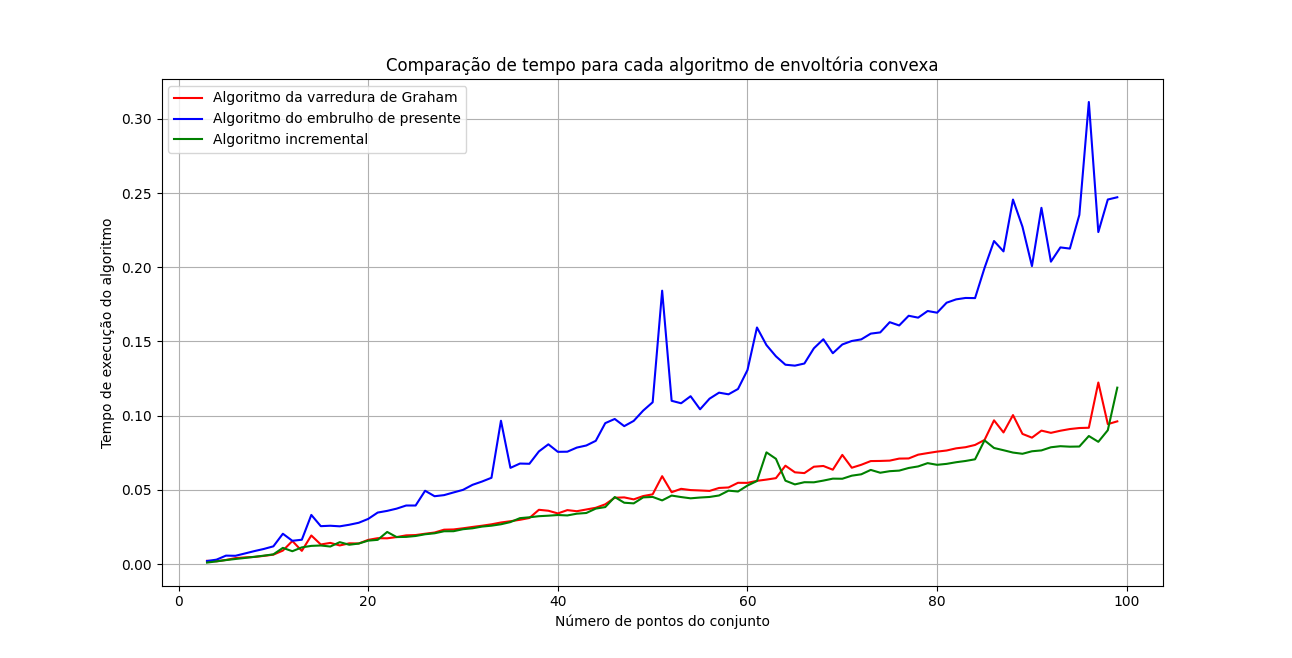
\includegraphics[width=12cm]{uniform.png}
	\centering
\end{figure}

O mesmo foi feito para pontos gerados aleatoriamente por uma distribuição exponencial, por meio da biblioteca \texttt{numpy}, com parâmetro escalar igual a \( \frac{1}{50} \), e obtivemos o seguinte resultado.

\begin{figure} [H]
	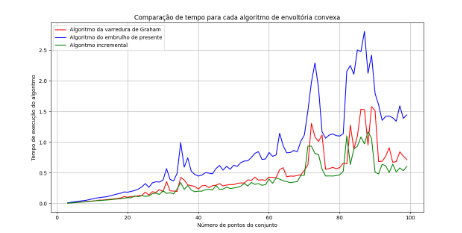
\includegraphics[width=9cm]{exponential.png}
	\centering
\end{figure}

Mais uma vez, tentamos uma distribuição diferente, disponível na biblioteca \texttt{numpy}, e desta vez geramos os pontos com uma distribuição normal de probabilidade, com média 50 e desvio padrão 10. O resultado segue abaixo:

\begin{figure} [H]
	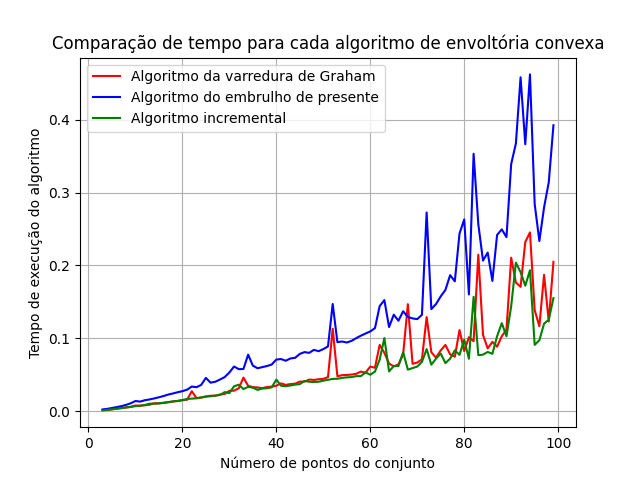
\includegraphics[width=9cm]{normal.png}
	\centering
\end{figure}

Podemos notar que em todos os casos o algoritmo incremental e o algoritmo da varredura de Graham tiveram tempos de execução muito similares, enquanto o algoritmo de embrulho de presente, por possuir pouca estabilidade e ser sensível à saída, teve um desempenho bem abaixo dos outros. Devemos, no entanto, analisar como cada um dos algoritmos se sai na prática com os pontos coletados pelo conjunto de dados que usaremos no trabalho.

De qualquer modo, podemos notar que eles seguem um padrão exatamente como esperávamos. A varredura de Graham e o algoritmo incremental, ambos com a mesma complexidade \( \Theta(n \log n) \), tiveram tempos de execução semelhantes para os testes feitos, enquanto o algoritmo do embrulho de presente demorou muito mais, dado sua inconsistência e sensibilidade à saída.

Após essas análises concluímos então que a melhor opção para utilizarmos no trabalho prático seria o algoritmo da varredura de Graham, uma vez que ela passou em todos os testes que criamos e apresentou um desempenho eficiente e consistente neles.

Adicionalmente esta classe possui um método para checar se uma envoltória convexa contém outra, dado que elas não se interceptam. Isso serve como checagem adicional para verificar a separabilidade linear: é possível que duas envoltórias não se interceptem, mas uma esteja dentro da outra, de tal maneira tornando a separação impossível.

Por fim, temos um método importante para o trabalho que retorna o segmento de menor tamanho entre o vértice de uma envoltória e um vértice de outra. Mais especificamente, para casos em que podemos separar linearmente as envoltórias, devemos seguir, conforme especifica o enunciado do trabalho, alguns passos para facilitar as computações. O primeiro deles é encontrar o segmento que une dois vértices, um de cada envoltória, de modo que a distância entre esses vértices seja a menor possível.

Sem nos alongarmos muito nesse quesito, mesmo quando as envoltórias não possuem interseção entre si, essa reta pode nos indicar que não podemos separar os dados linearmente segundo nossas especificações. Isso por quê estamos pegando a menor distância entre dois vértices e não a menor distância entre as envoltórias como um todo, o que daria muito mais trabalho.

De qualquer modo, abordamos a estratégia mais ingênua possível para encontrar essa reta. Para calcular o segmento supracitado, comparamos todos os pontos da envoltória 1 com todos os pontos da envoltória 2, de modo a encontrar aqueles com a menor distância. Com esses pontos encontrados, basta criarmos a instância de segmento que é formada pelos dois e retornarmos na função.

\subsubsection{Event}

Um evento, no contexto da varredura linear, é um ponto que pode gerar uma interseção de segmentos. Isto é, não é necessário implementar a varredura linear como uma linha contínua percorrendo o eixo \( x \), mas sim como saltos discretos em pontos específicos: os terminais dos segmentos, sendo necessário saber se são o extremo esquerdo ou direito.

A classe \texttt{Event} implementa essa estrutura. Em particular, cada \texttt{Event} possui 5 atributos: duas coordenadas indicando a posição do evento, um booleano indicando se é um segmento da esquerda ou da direita, um identificador, apontando para o polígono que contém o evento e o segmento associado. Embora a princípio toda essa parafernália possa parecer uma complicação desnecessária, todos os membros tem seu devido propósito (em particular os mais deslocados, vide o próprio segmento). Além dos atributos facilitarem a implementação da varredura linear, essa classe implementa um comparador importante para processar os eventos na ordem correta: o principal critério de comparação é o \( x \), usa-se a orientação como desempate (esquerda ou direita) e possivelmente o \( y \) como desempate secundário.

\subsubsection{LineSweep}

A varredura linear é um procedimento que, percorrendo um conjunto de segmentos a partir de um dado eixo, consegue identificar interseções entre os segmentos de forma eficiente (a depender das estruturas de dados). Nesta implementação, o conjunto de segmentos consiste nos segmentos que compõem os polígonos que formam as envoltórias convexas apresentadas anteriormente. É usado o eixo \( x \), percorrido da esquerda para a direita.

Quanto à especificidade da implementação, a principal função dessa classe, \texttt{do\_polygons\_intersect()}, recebe como parâmetros os dois polígonos e usa a varredura linear para verificar se eles possuem interseção. Naturalmente que, possíveis interseções dentro de um mesmo polígono não são consideradas interseções neste contexto. Para isso, os polígonos recebem identificadores para diferenciar se ocorreu um cruzamento dentro do próprio polígono.

Como mencionado na classe \texttt{Event}, o processamento do eixo é dado a partir dos eventos. Em especial, ao inserir um segmento (seu evento da esquerda), é checado se o segmento em questão intercepta seus vizinhos e, ao remover um segmento (evento da direita), é checado se seus vizinhos interceptam um ao outro. Desse modo, se faz necessário inverter o sentido de segmentos que apontam para a esquerda.

Para realizar as inserções e remoções de maneira eficiente, foi usada uma árvore AVL, da biblioteca \texttt{pytrees} (inclusa no código). A comparação dos pontos é feita a partir do \( x \) atual da varredura linear. Além disso, a referência \footcite{SL18} de implementação não considerava que um ponto poderia ser o início de mais de um segmento, o que é incompatível com trabalhar com polígonos. Para diferenciar segmentos que compartilham tal ponto, é usado um \( \epsilon \) na comparação, que permite que um deles se sobreponha sobre o outro.

Outra etapa importante é a função que calcula os vizinhos de um dado nodo. Essa função não estava implementada na biblioteca usada. Quando um nodo tem filhos, o nodo que melhor o aproxima por baixo é o maior da subárvore da esquerda e o que melhor aproxima por cima é o menor da subárvore da direita. Se algum dos filhos não existir, é necessário achar o primeiro ancestral que atenda a condição de ser menor ou maior que o nodo em questão. Apesar de caminhar em todos os níveis da árvore (no pior caso), como ela é balanceada, a complexidade é \( \Theta(\log n) \). Como comentado no código, apesar de essa função fazer mais sentido para uma árvore, averiguou-se adequado deixá-la nesta classe, por simplicidade.

Em relação ao custo geral do algoritmo, existem algumas operações lineares na soma do número de segmentos, como a criação do objeto \texttt{polygons} com os segmentos, a inversão e a população da lista de eventos. Mas no final, o gargalo é o laço principal, que para cada evento executa operações com, no máximo, custo logarítmico. Portanto a complexidade é \( \Theta(n \log n) \) no número de eventos (dobro da soma de segmentos).

Apesar de que um algoritmo mais simples pudesse ter sido desenvolvido dado que os segmentos em questão são originados a partir de dois polígonos convexos, optou-se por escrever um algoritmo mais genérico, que resolva (quase) todo tipo de interseção entre conjuntos de segmentos com identificadores.

\subsubsection{AlgorithmVisualization}

A classe \texttt{AlgorithmVisualization} não faz parte do escopo do trabalho, e foi feita apenas para que pudéssemos visualizar bem como os algoritmos estavam sendo executados, além de auxiliar na correção de bugs encontrados ao longo da execução.

Utilizamos a biblioteca \texttt{pygame}, uma biblioteca da linguagem Python destinada à criação de jogos simples, para a criação dessas animações. Optamos em utilizá-la para isso pois alguns integrantes da equipe já tinham familiaridade com a tecnologia e porque sua documentação é bem completa.

Todas as animações feitas foram dos três algoritmos de cálculo da envoltória convexa citados anteriormente. De forma geral, podemos dizer que ver uma animação da execução dos algoritmos foi crucial para que erros fossem identificados e conseguíssemos corrigir os \textit{bugs}.

Não vamos nos estender muito em relação à documentação dessa classe, visto que ela não fazia parte das definições no enunciado do trabalho. No entanto, deixaremos anexo à esta documentação um vídeo gravado por um de nossos integrantes demonstrando a visualização da execução dos algoritmos, além de que deixaremos ao final desta documentação instruções caso queiram rodar as animações localmente.

\subsubsection{Classifier}

A classe \texttt{Classifier} é a responsável pela criação do modelo de classificador proposto. Ao ser criada ela recebe dois vetores de pontos, da classe \texttt{Point}, que representam os dados de das classes, tendo um vetor os pontos de uma classe e o outro os pontos de outra classe. O objetivo final dessa classe é receber um ponto e classificá-lo de acordo com a reta proposta pelo modelo. Tendo em vista esse objetivo, a classe possui três funções:

{\begin{itemize}
	\item Função inicializadora que recebe duas listas do tipo \texttt{Point} e atribui os valores a serem guardados na classe de acordo com esses dados. Para isso, ela utiliza da função \texttt{fit()} para atribuir os valores da reta do modelo (função a ser abordada abaixo), além de atribuir os dados das listas para dentro da classe usando as listas internas \textit{class1} e \textit{class2} e salvar, por meio das varáveis class\_gt e class\_lt, qual subplano representa qual classe modelada.

	\item A função \texttt{fit()} é responsável por criar a reta do modelo. Ela procura os dois pontos que tem a menor distância euclidiana dentre os dados recebidos, com a restrição de que esses dois pontos devem ser de classes diferentes. Encontrados esses pontos, encontra-se, a partir da função \texttt{get\_perpendicular\_segment()} da classe \texttt{Segment}, o segmento de reta perpendicular ao segmento que liga esses dois pontos e que passa pelo seu ponto médio, criando assim a reta do modelo. Por fim, a função retorna os coeficientes angular e linear da reta criada além do ponto médio usado para criá-la que representa um ponto da reta.

	\item A função \texttt{test} é a função responsável por atingir o objetivo final da classe, para isso ela recebe um vetor do tipo \texttt{Point} e retorna a previsão da classe desses pontos de acordo com a reta modelada, ou seja, utiliza da coordenada \( x \) do ponto e dos coeficientes angular e linear da reta modelada para retornar qual a classe do ponto recebido, faz isso para todos os dados do tipo Point da lista recebida e retorna uma lista qual as classes respectivas a cada ponto.

\end{itemize}}

\section{Análise experimental dos dados}

\subsection{Bases de dados utilizadas}

Como descrito na especificação do trabalho, importamos e utilizamos no desenvolvimento do nosso trabalho 10 bases de dados extraídas do repositório de dados do software de análise de dados KEEL.

Buscamos utilizar ao menos 5 bases que continham dados linearmente separáveis. Também consideramos importante utilizar dados que não eram linearmente separáveis, justamente para ver a eficiência do nosso algoritmo em checar esses casos e também pois nem sempre, na prática, teremos dados funcionam perfeitamente como queremos.

De modo geral, estes foram os conjuntos de dados que utilizamos para nosso trabalho:

\begin{enumerate}
	\item Iris
	\item Glass
	\item Wine
	\item Newthyroid
	\item Segment
	\item Haberman
	\item Titanic
	\item Mammographic
	\item Banana
	\item Magic

\end{enumerate}

\subsection{Processamento dos dados}

Para computar todas as métricas definidas pelo escopo do trabalho, precisávamos converter os dados lidos nas bases de dados para tipos que se encaixam em nossa implementação. Para isso, portanto, um primeiro passo para cada conjunto foi transformar os dados no tipo Point, definido nas seções anteriores.

O segundo passo consistiu em dividir os dados obtidos no primeiro passo em duas partes. Uma que continha 70\% dos dados presentes na base de dados, que será utilizada para o treinamento e criação do classificador. Os outros 30\% serão então utilizados para analisar o desempenho do modelo de classificação. Essa separação é feita de forma pseudo aleatória, por meio da biblioteca \texttt{Pandas}, utilizada para leitura dos arquivos que continham os dados.

Alguns dados precisam de processamento adicional para que a gente possa classificar, como o conjunto Íris, que possui mais de duas classes separando suas instâncias. No entanto, acreditamos não ser necessário discorrer aqui sobre como cada uma dessas bases de dados foi processada especificamente.

Com esses conjuntos de dados bem separados e definidos, é possível prosseguir com o trabalho e prosseguir com os treinamentos e testes.

\subsection{Treinamento do classificador}

Nessa seção, vamos falar especificamente sobre como foi o treinamento do classificador para cada conjunto de dados, disponibilizando em cada subseção as imagens gráficas das envoltórias criadas, podendo assim visualizar quando os dados são linearmente separáveis ou não.

\subsubsection{Iris}

O conjunto de dados Iris é um conjunto de dados em particular que possui mais de duas classes de separação. Optamos então por separar as classes entre aquelas instâncias que pertencem à 'Iris-Setosa' e aqueles que não.

Além disso, cada instância da base de dados possui 4 atributos principais que os definem, sendo eles largura e comprimento de sépalas e pétalas. Para nosso classificador, utilizamos apenas os valores de largura e comprimento de pétalas, podendo assim produzir pontos bidimensionais.

Ao executar o código após o processamento dos dados, tivemos como resposta que nossos dados eram linearmente separáveis e obtivemos o seguinte gráfico:

\begin{figure} [H]
	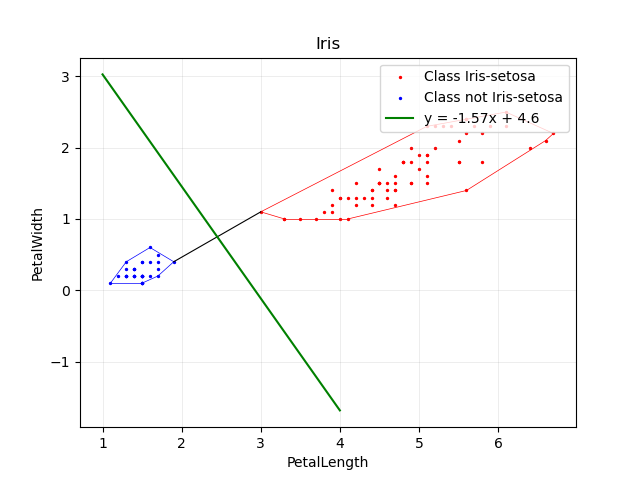
\includegraphics[width=12cm]{iris.png}
	\centering
\end{figure}

Podemos ver claramente pela imagem que os dados são de fato separáveis linearmente.

\subsubsection{Wine}

A base de dados Wine possui separabilidade quando escolhemos as classes 1 e 3 no conjunto de dados, e utilizamos os atributos \textit{TotalPhenols} e \textit{flavanoids} como as coordenadas dos pontos que serão gerados.

Nosso código, portanto, nos retorna que os dados são linearmente separáveis e temos o seguinte gráfico gerado:

\begin{figure} [H]
	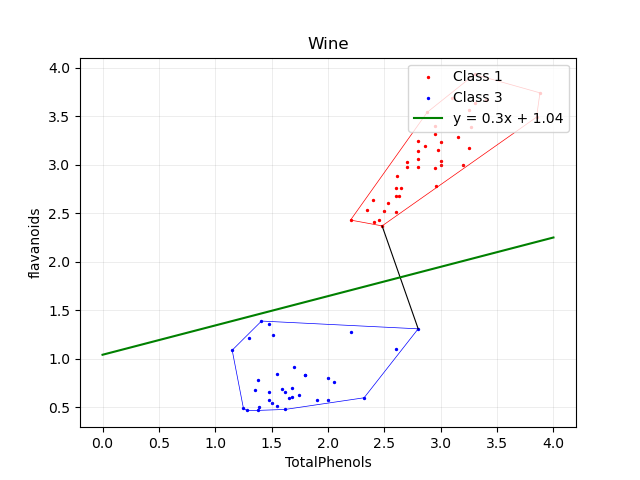
\includegraphics[width=12cm]{wine.png}
	\centering
\end{figure}

\subsubsection{Glass}

O conjunto de dados Glass possui uma grande quantidade de atributos para cada instância, as quais são divididas em 7 classes diferentes. De modo a gerarmos um conjunto de dados que pudesse ser separável que pudéssemos utilizar nossos classificadores, escolhemos especificamente os atributos Na e Mg como eixos do nosso sistema de coordenadas, e escolhemos as classes 1 e 3 para serem separadas.

Nosso sistema nos responde que os dados são separáveis, e temos o seguinte gráfico gerado:

\begin{figure} [H]
	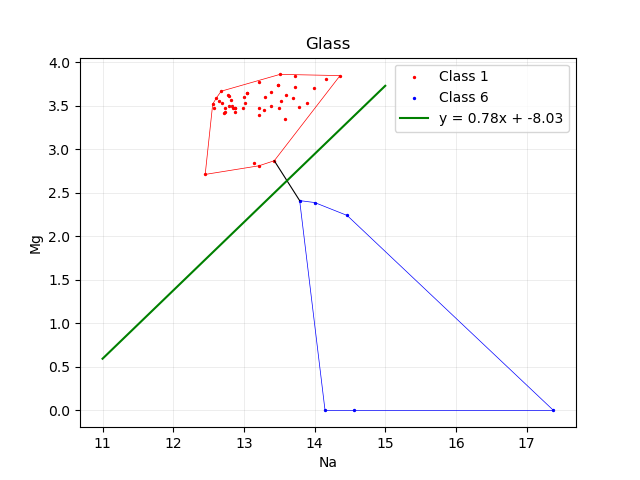
\includegraphics[width=12cm]{glass.png}
	\centering
\end{figure}


\subsubsection{Newthyroid}

A base de dados \textit{Newthyroid} também é separável, se escolhermos como coordenadas os atributos \textit{Thyroxin} e \textit{TSH\_value}, e como classes as classes 2 e 3. Ao executarmos o código, não identificamos intersecção entre as envoltórias e temos o seguinte gráfico:

\begin{figure} [H]
	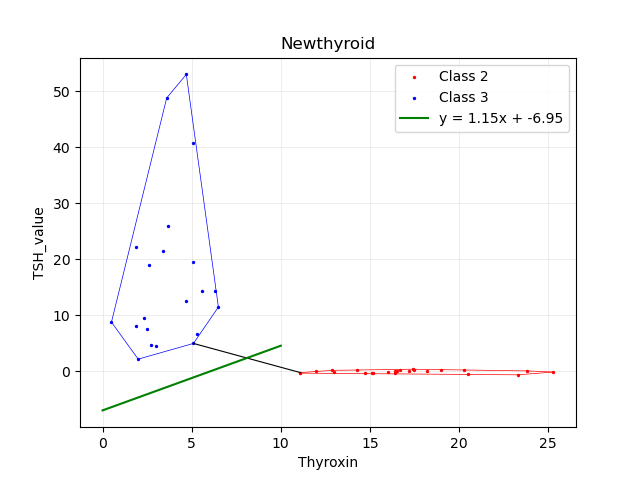
\includegraphics[width=12cm]{newthyroid.png}
	\centering
\end{figure}

\subsubsection{Segment}

Mais uma base que pudemos identificar como separável foi o conjunto de dados Segment. Ela possui instâncias com uma grande quantidade de atributos, divididas entre 7 classes. Para garantir a separabilidade, utilizamos os atributos \textit{Region-centroid-col} e \textit{Rawblue-mean} como coordenadas do plano cartesiano, e separamos pelas classes 1 e 2.

Nosso sistema nos retornou que nossos dados eram linearmente separáveis, e obtivemos o seguinte gráfico resultante:

\begin{figure} [H]
	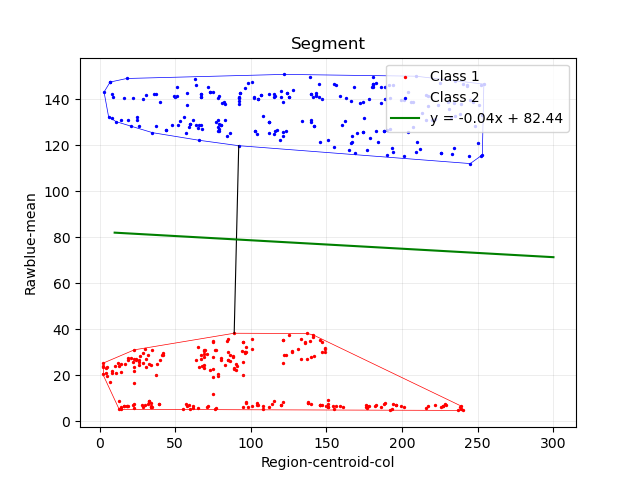
\includegraphics[width=12cm]{segment.png}
	\centering
\end{figure}

\subsubsection{Titanic}

O conjunto de dados Titanic, por sua vez, não era separável. Qualquer escolha de seus atributos como coordenadas dos pontos não permitia uma separação linear entre as envoltórias criadas. Nossa implementação, portanto, sempre retornava que os dados não podiam ser separados.

Obtivemos o seguinte gráfico gerado, utilizando os atributos \textit{Class} e \textit{Age} como as coordenadas:

\begin{figure} [H]
	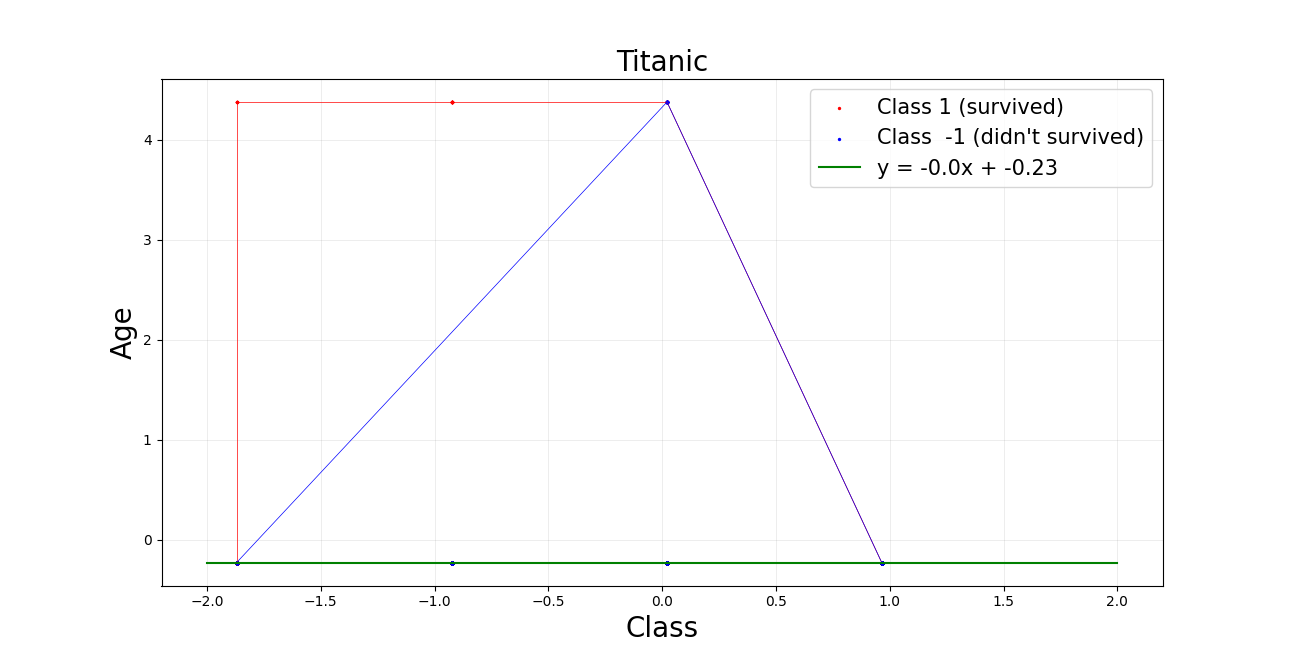
\includegraphics[width=12cm]{titanic.png}
	\centering
\end{figure}

\subsubsection{Mammographic}

A base de dados Mammographic é mais uma que não possui separabilidade linear dos dados, independente das escolhas de atributos como coordenadas dos pontos. Para demonstrar isso visualmente aqui, escolhemos \textit{Age} e \textit{Density} como as coordenadas, pois nesse caso temos uma situação especial em que as duas envoltórias compartilham vértices.

Obtivemos, então, o seguinte gráfico:

\begin{figure} [H]
	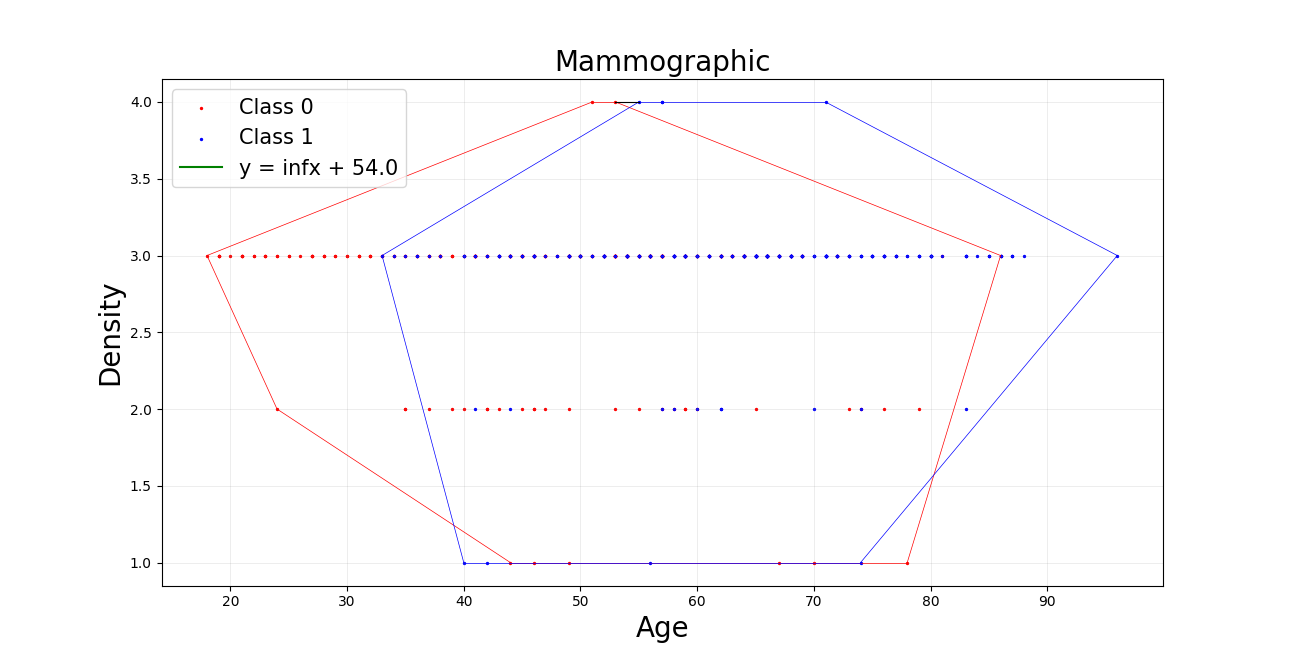
\includegraphics[width=12cm]{mammographic.png}
	\centering
\end{figure}

\subsubsection{Banana}

O conjunto de dados Banana é uma ótima base para o trabalho, uma vez que possui apenas dois atributos que podem representar as duas dimensões dos pontos, assim como apenas duas classes, permitindo um bom teste de separação.

Ao executar o código, nossa implementação nos respondeu que os dados não eram linearmente separáveis, e pudemos ver isso claramente pelo seguinte gráfico. Portanto, não havia como utilizá-lo no classificador.

\begin{figure} [H]
	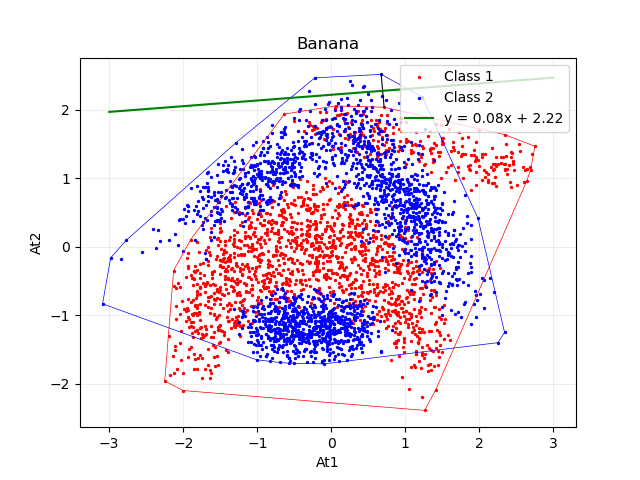
\includegraphics[width=12cm]{banana.png}
	\centering
\end{figure}

\subsubsection{Magic}

O conjunto de dados Magic é bem confuso e possuía grande quantidade de atributos. Por ser mais fácil de compreender e manipular, escolher os atributos \textit{FLenght} e \textit{FWidth} como as coordenadas de nossos pontos no plano cartesiano. A base de dados é separada em duas classes, g e h, o que facilitou a checagem das separações.

Com a execução do código, tivemos a resposta de que os dados não são linearmente separáveis, e podemos ver isso no seguinte gráfico:

\begin{figure} [H]
	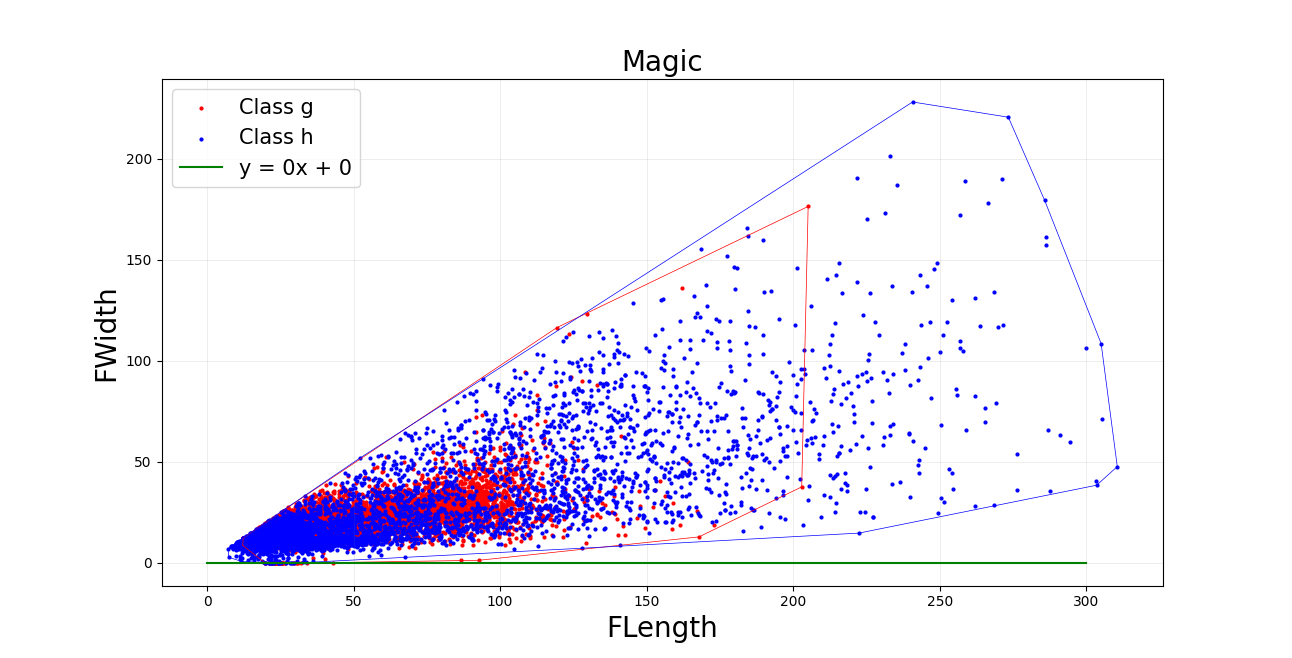
\includegraphics[width=12cm]{magic.png}
	\centering
\end{figure}

\subsubsection{Haberman}

O conjunto de dados Haberman apresenta duas classes, sendo elas Positive ou Negative, assim como três atributos. Testamos para todas as três combinações de atributo como coordenadas de pontos e em todos os casos os dados continuaram não sendo linearmente separáveis, segundo nosso algoritmo.

No gráfico abaixo, utilizamos os atributos \textit{Age} e \textit{Positive} como coordenadas. Podemos ver de forma clara que as envoltórias de cada classe se interceptam, o que implica que os dados não são separáveis linearmente.

\begin{figure} [H]
	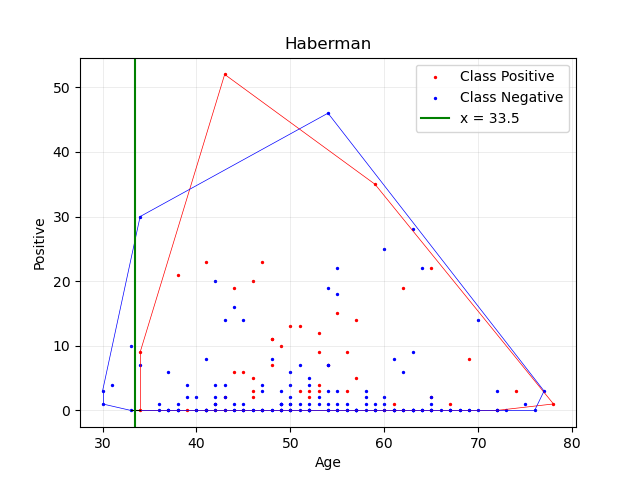
\includegraphics[width=12cm]{haberman.png}
	\centering
\end{figure}

\subsection{Análise de métricas}

Após gerarmos os gráficos e analisarmos os 10 conjuntos de dados escolhidos, necessitávamos analisar as métricas de separação linear, utilizando a biblioteca Scikit-Learn da linguagem Python.

Para cada base

\section{Conclusão}

O Trabalho Prático, de forma geral, foi extremamente importante para compreensão e estudo dos principais conceitos de geometria computacional aprendidos na disciplina.

A implementação de três algoritmos de envoltória convexa permitiu que notássemos as principais diferenças entre eles, principalmente em relação aos tempos de execução. A aplicação das primitivas de geometria computacional nessas implementações também foi consideravelmente importante para compreender o tema de forma geral.

A varredura linear, por sua vez, tomou um pouco mais de tempo do nosso grupo. A parte mais complicada certamente se refere ao uso de uma AVL no algoritmo, uma vez que muitos casos específicos precisavam ser considerados na hora de analisarmos se um segmento estava acima ou abaixo do outro. No entanto, após vários testes fomos capazes de consertar nosso algoritmo e finalizamos a implementação.

Após isso, tínhamos como tarefa a implementação do classificador, de modo a criar um sistema simples de aprendizado de máquina. A falta de familiaridade dos nossos membros com alguns conceitos de ciência de dados foi um empecilho no começo, mas com o tempo fomos capazes de aprender os conceitos e aplicá-los ao trabalho.

Em resumo, o trabalho foi muito interessante num ponto de vista de aprendizado. Colocar em prática tudo que foi aprendido certamente fez uma grande diferença para assimilar os conceitos.

\printbibliography

\end{document}
